\section{Black hole entropy: the entropy function and small black holes}\label{sec:entropy}

\subsection{The entropy function}\label{ssec:entropyfunction}

For an extremal black hole in a theory of gravity with covariant higher-derivative terms in the framework specified below, whose near-horizon geometry has the symmetry $SO(2,1)\times SO(D-1)$ of $AdS_2\times S^{D-2}$ with electric fields $e_i$ and magnetic charges $p_a$, Sen \cite{Sen05entropy} defined the entropy function
\begin{equation}\label{eq:entropyfunction}
\begin{gathered}
\mathcal E(\vec u,\vec v,\vec e,\vec q,\vec p) = 2\pi\big(e_i q_i - f(\vec u,\vec v,\vec e,\vec p)\big),\\
f = \int_{S^{D-2}}\sqrt{-\det g}\,\mathcal L ,
\end{gathered}
\end{equation}
where $f$ is the Lagrangian density integrated over the sphere on the near-horizon ansatz with radii $v_1,v_2$ of $AdS_2$ and $S^{D-2}$ and constant scalars $u_s$.

\begin{theorem}[claims 24, 25]\label{thm:entropyfunction}
\begin{enumerate}[label=(\roman*),leftmargin=2em]
\item The equations of motion of the near-horizon geometry are the conditions
\[
\partial\mathcal E/\partial u_s = \partial\mathcal E/\partial v_{1,2} = 0,\qquad \partial\mathcal E/\partial e_i = 0,
\]
the last being the definition of the charges $q_i$, and the Wald entropy of the black hole is the value of $\mathcal E$ at the extremum \cite{Sen05entropy}.
\item For rotating extremal black holes, whose near-horizon geometry has the symmetry $SO(2,1)\times U(1)$ and depends on the polar angle through functions $\Omega(\theta),\psi(\theta),\dots$, the same holds with $\mathcal E$ a functional of these functions and with an additional term $2\pi\alpha J$ for the angular momentum, the extremisation being over the functions as well as the constants \cite{AGJST06}.
\end{enumerate}
\end{theorem}

\begin{proof}
The derivation, including the normalization and curvature-variation convention, is given in \cite[Section~2]{Sen05entropy} and its rotating extension in \cite{AGJST06}. For a covariant Lagrangian with no derivatives of curvature, the Wald expression is $-2\pi\int_H (\partial\mathcal L/\partial R_{\mu\nu\rho\sigma})\epsilon_{\mu\nu}\epsilon_{\rho\sigma}$ with the induced volume factor and $\epsilon_{\mu\nu}\epsilon^{\mu\nu}=-2$. Curvature derivatives require the corresponding variational derivative, and Chern--Simons terms require separate treatment. The near-horizon equations and the Legendre transform give the entropy function in this framework. Local extremisation does not by itself construct a regular solution extending to prescribed asymptotic data.
\end{proof}

\begin{verdict}[claims 24, 25]
Proved. The theorem is a derivation within classical higher-derivative gravity with the stated symmetry; the attractor mechanism, that the entropy is independent of the asymptotic moduli, is a corollary whenever the extremum is isolated in the scalars. The results agree with the earlier supergravity computations of Cardoso, de Wit and Mohaupt where both apply \cite{Sen05entropy}, and the formalism has been used in every later comparison of macroscopic and microscopic entropies.
\end{verdict}

\subsection{Small black holes}\label{ssec:small}

A half-BPS state of the heterotic string on $T^6$ with winding $w$ and momentum $n$ on a circle, with $nw>0$, has $d_h(nw)\sim e^{4\pi\sqrt{nw}}$ states, while the two-derivative supergravity solution with these charges has a singular horizon of zero area. Sen \cite{Sen04stretch} argued that the higher-derivative terms stretch the horizon to string scale and that the entropy function with the Gauss--Bonnet term, $\mathcal L \supset \frac{1}{16\pi G}\phi(S)\big(R_{\mu\nu\rho\sigma}^2 - 4R_{\mu\nu}^2 + R^2\big)$ with the one-loop coupling $\phi(S)$, gives
\begin{equation}\label{eq:small}
S_{\rm BH} = 4\pi\sqrt{nw}
\end{equation}
in four dimensions, in agreement with the statistical entropy to leading order; \cite{Sen05stretching} extended the computation to the heterotic string in $D$ dimensions.

Sen states the outcome of the computation of \cite{Sen05stretching} in its abstract:
\begin{quote}\small
``The black hole entropy computed this way is finite and has the right dependence on the charges in accordance with the general scaling argument, but the overall numerical factor does not agree with that computed from the statistical entropy except for $D=4$ and $D=5$. This is not surprising in view of the fact that we do not use a fully supersymmetric action in our analysis; however this analysis demonstrates that higher derivative corrections are capable of stretching the horizon of a small black hole in arbitrary dimensions.''
\end{quote}
His result is \cite[Eq.~(3.20)]{Sen05stretching}, with the Gauss--Bonnet coefficient $C$ of his~(3.14),
\begin{equation}\label{eq:sen320}
S_{\rm BH}=a\sqrt{nw},\qquad a=\pi\sqrt C\sqrt{\frac{2}{(D-2)(D-3)}}\,\big\{8(D-2)(D-3)-4(D-4)(D-5)\big\}^{1/2}.
\end{equation}
Prester \cite{Prester06} then showed that the Lovelock action with the coefficients $\lambda_m=4^{1-m}/m!$ of his equation~(4.27) has, in every dimension, a near-horizon solution with $S_{\rm BH}=4\pi\sqrt{nw}$, and that his solution is unique for $D\le9$ \cite[footnote~9]{Prester06}. The rest of this subsection makes these statements exact for every dimension.

\paragraphx{The two-charge horizon.} We use the normalisation of \cite[Eq.~(4.3)]{Prester06}, with $n_D=D-2$ the dimension of the sphere and $\alpha'=1$ unless $\alpha'$ is written. The near-horizon geometry is $AdS_2\times S^{n_D}$ with squared radii $v_1,v_2$, the string-frame dilaton is $u_S$, the radius of the circle is $u_T$, and $e_1,e_2$ are the electric fields of the momentum and winding charges $q_1=2n/\sqrt{\alpha'}$, $q_2=2w/\sqrt{\alpha'}$. For a tree-level action whose higher-derivative terms are built from the Riemann tensor alone,
\begin{equation}\label{eq:fgeneral}
f=K\,u_S\,v_1v_2^{n_D/2}\Big[\frac{2(u_T^2e_1^2+e_2^2u_T^{-2})}{v_1^2}+Q(v_1,v_2)\Big],
\end{equation}
where $K>0$ is a constant and $Q$ is the curvature Lagrangian on the product of radii $v_1,v_2$; for the Einstein term $Q=n_D(n_D-1)/v_2-2/v_1$.

\begin{theorem}[entropy of the two-charge horizon]\label{thm:twocharge}
Let $R(v_1,v_2)=-v_1^2\,Q(v_1,v_2)$. The near-horizon solutions with $v_1,v_2,u_S,u_T,e_i>0$ are in bijection with the critical points of $R$ in the positive quadrant at which $R>0$, and at such a point
\begin{equation}\label{eq:sR}
S_{\rm BH}=4\pi\sqrt{nw}\,\sqrt{R_*/\alpha'}.
\end{equation}
In particular the black hole entropy equals the statistical entropy $4\pi\sqrt{nw}$ if and only if $R_*=\alpha'$, which is the condition $e_1e_2=\alpha'/4$ of \cite[Eq.~(5.6)]{Prester06}.
\end{theorem}

The proof is in Appendix~\ref{app:closures}. The theorem reduces the comparison with the statistical entropy, for every action of this class, to a single number: the critical value of a function of two variables. For the Lovelock actions $\mathcal L=\sum_m\lambda_m\alpha'^{m-1}\mathcal L_m^{GB}$ with $\lambda_1=1$ the function \eqref{eq:fgeneral} is that of \cite[Eq.~(4.3)]{Prester06}, and
\begin{equation}\label{eq:GH}
Q=H(v_2)-\frac{G(v_2)}{v_1},\quad G(y)=\sum_{m\ge1}\frac{2m\lambda_m\,n_D!}{(n_D+2-2m)!}\,y^{1-m},\quad H(y)=\sum_{m\ge1}\frac{\lambda_m\,n_D!}{(n_D-2m)!}\,y^{-m},
\end{equation}
the sums running over the terms with nonnegative factorial arguments.

\begin{corollary}[Lovelock actions]\label{cor:lovelock}
For a Lovelock action the near-horizon solutions correspond to the critical points $y$ of $\Phi=G^2/H$ on the set where $G>0$ and $H>0$, with $v_2=\alpha'y$, $v_1=\alpha'G/(2H)$ and $S_{\rm BH}=2\pi\sqrt{nw\,\Phi(y)}$. The statistical value is $\Phi=4$.
\end{corollary}

\begin{corollary}[the Gauss--Bonnet truncation in closed form]\label{cor:gb}
For $\lambda_2=1/8$ and $\lambda_m=0$ for $m\ge3$, with $a=(D-2)(D-3)$ and $b=(D-4)(D-5)$, there is exactly one near-horizon solution in every dimension $D\ge4$. It has $v_2=\alpha'(a-b)/4$, $v_1=2v_2/a$ and
\begin{equation}\label{eq:gbratio}
\frac{S_{\rm BH}}{4\pi\sqrt{nw}}=\sqrt{1-\frac{(D-4)(D-5)}{2(D-2)(D-3)}}.
\end{equation}
The ratio is $1$ for $D=4,5$, it is $\sqrt{11/12}$, $\sqrt{17/20}$, $\sqrt{4/5}$ for $D=6,7,8$, and it decreases to $1/\sqrt2$ as $D\to\infty$. It is the ratio $a_D/a_4$ of Sen's coefficients \eqref{eq:sen320}, for every value of $C$.
\end{corollary}

The corollary turns Sen's statement into a formula with its domain: the Gauss--Bonnet truncation fixes the horizon in every dimension, the entropy is below the statistical value for every $D\ge6$, and it never falls below $1/\sqrt2$ of it.\footnote{Sen prints \eqref{eq:sen320} with $C=1$ beside it, while his~(3.15) gives $C=1/8$ for the heterotic string; the two differ by the choice of $\alpha'$. Since $a\propto\sqrt C$, the ratio $a_D/a_4$ does not depend on this choice, and $a_4=4\pi$ by Sen's own statement fixes the normalisation.} The solution is the minimum of $\Phi$, and the critical point equation is linear in $1/y$, which is why it can be solved in every dimension.

\begin{theorem}[Prester's completion in every dimension]\label{thm:prester}
Let $\lambda_m=4^{1-m}/m!$ for every $m\ge1$, and $D\ge4$.
\begin{enumerate}[label=(\roman*),leftmargin=2em]
\item $H=2(G-2)$ identically, in every dimension. Equivalently $f$ has the form \cite[Eq.~(5.3)]{Prester06}.
\item On the line $v_1=\alpha'/2$ one has $R(\alpha'/2,v_2)=\alpha'$ for every $v_2$, and every near-horizon solution lies on this line. Hence every solution has $S_{\rm BH}=4\pi\sqrt{nw}$.
\item The near-horizon solution is unique: $v_2=\alpha'y_D$ with $y_D$ the only positive root of $H(y)=4$. Equivalently $I_{n_D}\big(1/(2y_D)\big)=2$, where
\[
I_N(t)=\sum_{m\ge0}\binom{N}{2m}(2m-1)!!\,t^m
\]
counts the involutions of an $N$-element set with weight $t$ per transposition, or again $i^{-n_D}\operatorname{He}_{n_D}\big(i\sqrt{2y_D}\big)=2(2y_D)^{n_D/2}$ with $\operatorname{He}_N$ the Hermite polynomial.
\item As $D\to\infty$, with $n_D=D-2$,
\[
y_D=\frac{n_D^2}{4\ln2}-\frac{(2\ln2+1)\,n_D}{4\ln2}+O(1).
\]
\end{enumerate}
\end{theorem}

Part~(ii) for one solution is Prester's argument of \cite[Section~5]{Prester06}, which he gives without solving for $v_2$; parts~(i) and~(ii) show that it applies to every solution, because $\partial_{v_2}R=v_1G'(v_2)(1-2v_1)$ and $G'<0$. Part~(iii) extends his uniqueness statement from $D\le9$ to every dimension, and part~(iv) refines the leading term $v_2\to D^2\alpha'/(4\ln2)$ of \cite[Eq.~(20)]{Prester13}. The first values are $y_4=1/2$, $y_5=3/2$, $y_6=3/2+\sqrt3$, and $y_{40}=489.273\dots$

\begin{theorem}[the coefficients are forced]\label{thm:rigidity}
Fix $D\ge4$, let $m=\lfloor D/2\rfloor$, and take $\lambda_k=4^{1-k}/k!$ for $k<m$ and $\lambda_m=\beta\,4^{1-m}/m!$ with $\beta>0$.
\begin{enumerate}[label=(\roman*),leftmargin=2em]
\item The coefficient $\lambda_m$ enters $G$ and not $H$, and $\Phi_\beta=G_\beta^2/H$ attains its minimum on $(0,\infty)$.
\item If $\beta>1$, every near-horizon solution has $S_{\rm BH}>4\pi\sqrt{nw}$.
\item If $\beta<1$, the solution at the minimum of $\Phi_\beta$ has $S_{\rm BH}<4\pi\sqrt{nw}$.
\end{enumerate}
Consequently, if $\lambda_1=1$, every $\lambda_k$ is positive, and the solution at the minimum of $\Phi$ has the statistical entropy in every dimension, then $\lambda_k=4^{1-k}/k!$ for every $k$.
\end{theorem}

The induction in the last statement uses that $\lambda_m$ is the top coefficient both in $D=2m$ and in $D=2m+1$: it is fixed by $D=2m$, and Theorem~\ref{thm:prester} shows that the same value works in $D=2m+1$. This proves the statement of \cite{Prester13} that the matching ``fixes the coefficients $\lambda_k$ to the form (6) uniquely'', which there rests on the computations of \cite{Prester06}. Figures~\ref{fig:valley} and~\ref{fig:rigidity} show the two mechanisms: a line of constant $R$ on which every solution lies, and a minimum that crosses the statistical value only at $\beta=1$.

\begin{figure}[tbp]
\centering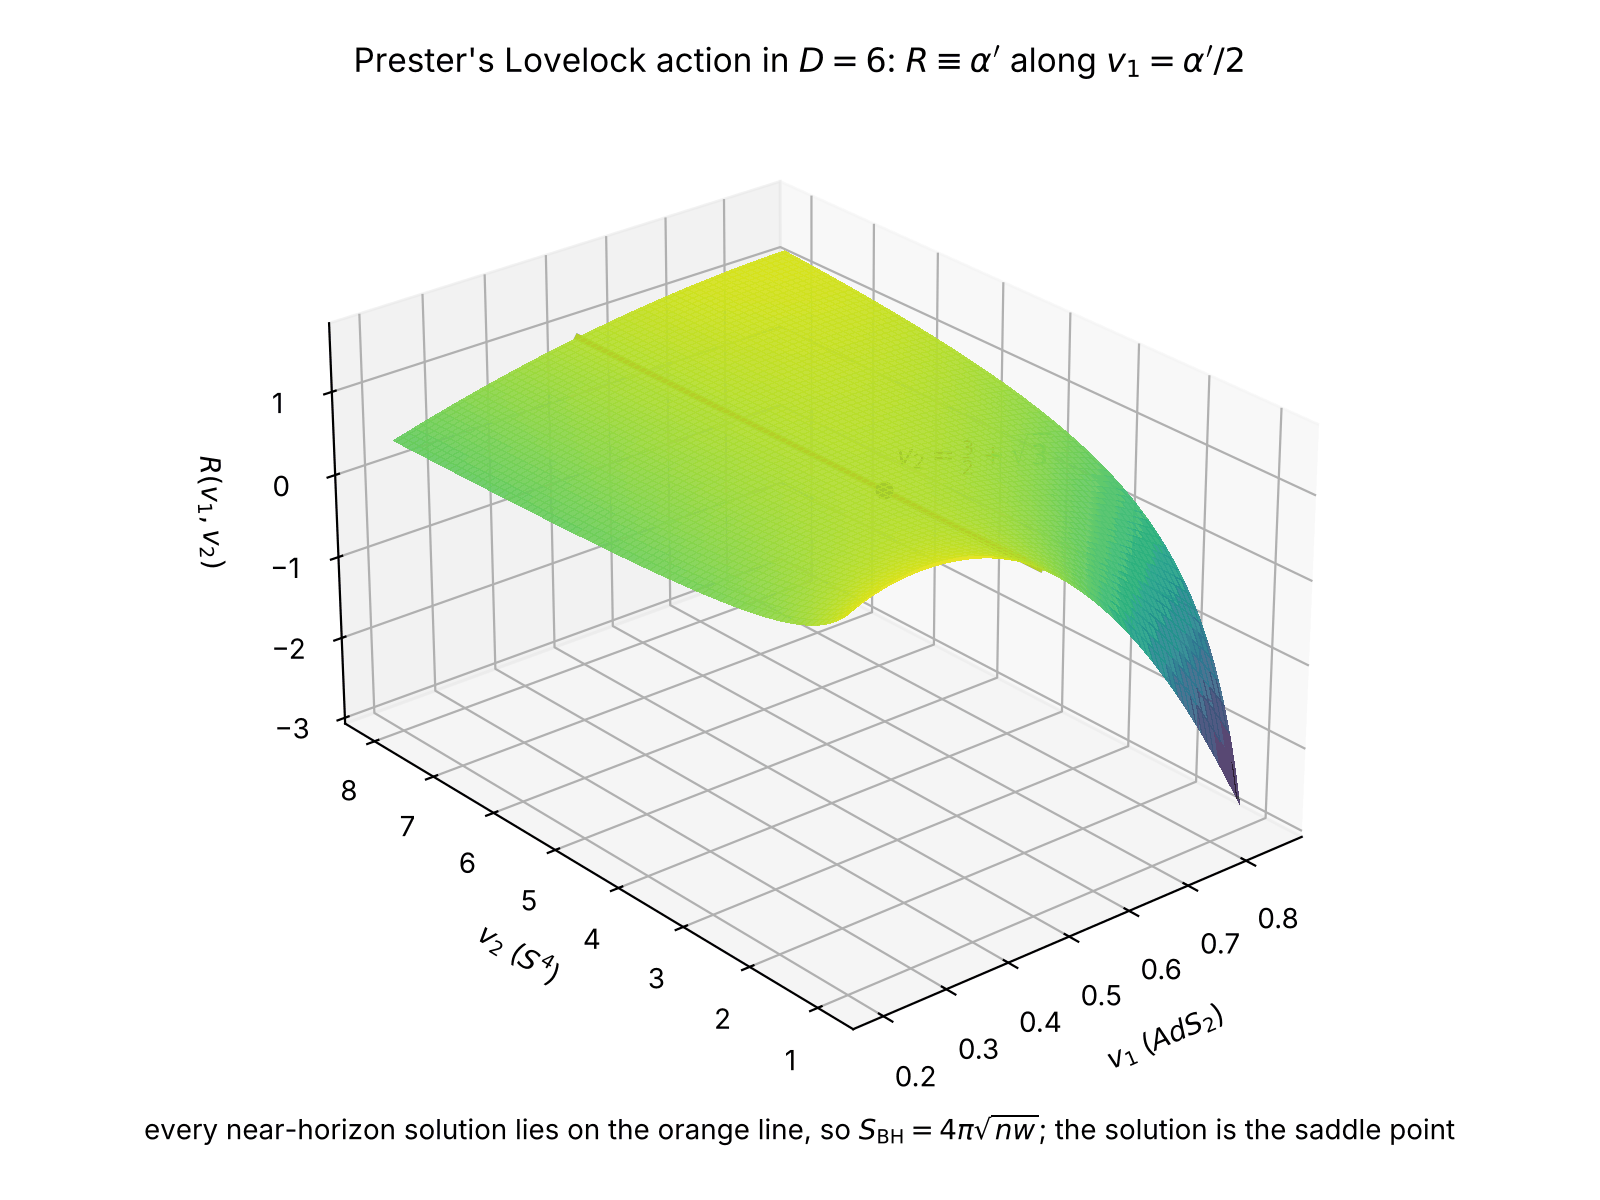
\includegraphics[width=0.94\linewidth,height=0.46\textheight,keepaspectratio]{figures/fig_valley.png}
\caption{The function $R(v_1,v_2)$ of Theorem~\ref{thm:twocharge} for Prester's coefficients in $D=6$, in units $\alpha'=1$. Along the line $v_1=1/2$ (orange) the surface has the constant height $R=1$, the value that gives $S_{\rm BH}=4\pi\sqrt{nw}$; the near-horizon solution is the saddle point on this line, at $v_2=3/2+\sqrt3$.}
\label{fig:valley}
\end{figure}

\begin{figure}[tbp]
\centering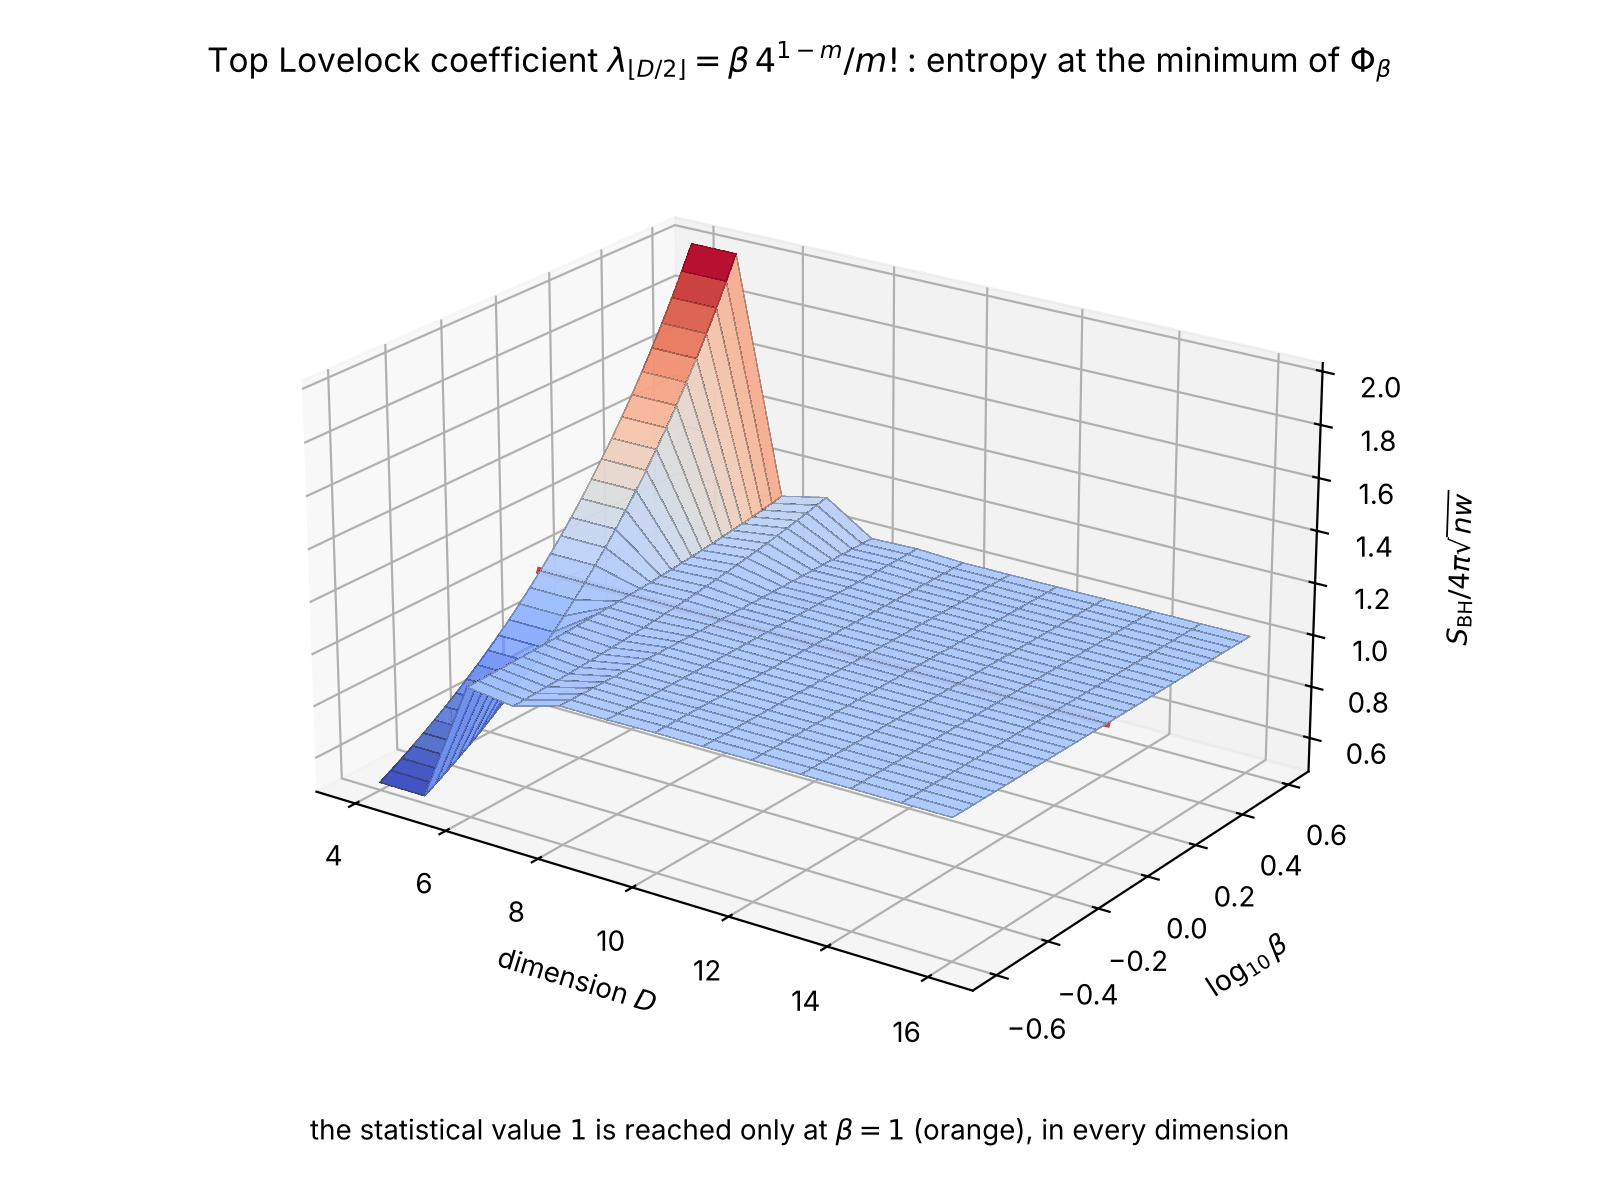
\includegraphics[width=0.94\linewidth,height=0.46\textheight,keepaspectratio]{figures/fig_rigidity.png}
\caption{The entropy at the minimum of $\Phi_\beta$, divided by $4\pi\sqrt{nw}$, as a surface over the dimension $D$ and the factor $\beta$ of the top Lovelock coefficient (Theorem~\ref{thm:rigidity}). The level $1$ is met only along $\beta=1$ (orange): above it the entropy exceeds the statistical value, below it the entropy falls short.}
\label{fig:rigidity}
\end{figure}

\begin{remark}[four dimensions]\label{rem:fourd}
In $D=4$ the agreement extends to all orders in $1/\sqrt{nw}$ when the supersymmetric $F$-terms are used in place of the Gauss--Bonnet term: \cite{Dabholkar05} evaluated the entropy with the full $F$-term, and \cite{DDMP05} matched it with the asymptotic expansion of $d_h$ up to non-perturbative terms. The Gauss--Bonnet term reproduces the leading term because on the near-horizon geometry the four-dimensional $F$-term reduces to it at this order.
\end{remark}

\begin{remark}[what remains open for the heterotic string]\label{rem:heterotic}
\gap{The heterotic effective action in $D\ge6$ is not the Lovelock action.} It contains no cubic Gauss--Bonnet density, its quartic terms carry $\zeta(3)$, and it has higher-derivative terms in the gauge fields \cite[Section~6]{Prester06} and gravitational Chern--Simons terms \cite[footnote~6]{Prester13}. Theorem~\ref{thm:twocharge} still applies to its pure-curvature part, so the open question is the single statement $R_*=\alpha'$ for the complete action on $AdS_2\times S^{D-2}$, and that requires the full $\alpha'$ expansion, which is not known. The holographic arguments of \cite{DM08,KLS07,LSS07}, which obtain the entropy from the central charge of an $AdS_3$ near-horizon region fixed by symmetries and anomalies, support the statistical value in every dimension; they do not compute $R_*$ from an action.
\end{remark}

\begin{verdict}[claim 26]
Proved, for the statements Sen makes. The Gauss--Bonnet truncation gives a finite horizon in every dimension, with the entropy \eqref{eq:gbratio} in closed form, equal to the statistical value exactly for $D=4,5$ (Corollary~\ref{cor:gb}). For every action whose corrections are built from curvature, the comparison is the single condition $R_*=\alpha'$ (Theorem~\ref{thm:twocharge}); Prester's Lovelock completion satisfies it with a unique solution in every dimension, and its coefficients are the only ones that do (Theorems~\ref{thm:prester} and~\ref{thm:rigidity}). The statement that the complete heterotic effective action gives $4\pi\sqrt{nw}$ in every $D\ge6$ remains open (Remark~\ref{rem:heterotic}).
\end{verdict}
